\chapter{Evaluation Results}\label{evaluation-results}

\minitoc

This chapter presents the effectiveness of the VV Python library in
improving healthcare data visualization for academic research. We
compare its performance against traditional methods. Our focus is on two
metrics: "Time-to-First-Chart Draft" and "Time-to-Final-Chart."

The data for this evaluation was collected from a project that involved
producing visual representations from a set of 72 spreadsheets. These
times were captured using Monday.com, following a well-established
practice within the organization where the author works for project
management, including time-tracking. Time measurements for VV were taken
using Python\textquotesingle s time library, by calculating the delta of
time between the start and completion of relevant tasks.

\section{Time Decomposition}\label{time-decomposition}

The total time to complete the project was decomposed into two main
categories:

\textbf{Initial Setup Time}

\begin{itemize}
\item
  For a human analyst, this refers to the time spent on organizing the
  spreadsheets and preparing the necessary files for task completion.
\item
  For the VV system, this means the time required for adequately setting
  up the software environment and data linkage.
\end{itemize}

\textbf{Time per Spreadsheet}

\begin{itemize}
\item
  This is the time taken to generate a chart from each individual
  spreadsheet.
\end{itemize}

\section{Time Metrics}\label{time-metrics}

\begin{table}[]
  \caption{Time Metrics Comparing Manual Methods and VV Python Library for a Project with 72 Spreadsheets.}
  \label{tab:times}
  \begin{tabular}{llcc}
  \hline
  \multicolumn{1}{c}{\textbf{Metric}}                 & \textbf{}                             & \textbf{\begin{tabular}[c]{@{}c@{}}Manual\\ Methods\end{tabular}} & \textbf{Visual Viper}                                                                 \\ \hline
  \multirow{3}{*}{\textbf{Time-to-First-Chart-Draft}} & \textbf{Initial setup}                & 0h30min                                                           & 2h00min                                                                               \\ \cline{2-4}
                                                      & \textbf{Time per spreadsheet}         & 5min                                                              & \textless{}10\textsuperscript{-3}                                                                       \\ \cline{2-4}
                                                      & \textbf{Total time (72 spreadsheets)} & 6h30min                                                           & 2h00min                                                                               \\ \hline
  \multirow{3}{*}{\textbf{Time-to-Final-Chart}}       & \textbf{Initial setup}                & 0h30min                                                           & 2h00                                                                                  \\ \cline{2-4}
                                                      & \textbf{Time per spreadsheet}         & 12min                                                             & \begin{tabular}[c]{@{}c@{}}To Miro: $\sim$4 sec\\ To GDrive: $\sim$3 sec\end{tabular} \\ \cline{2-4}
                                                      & \textbf{Total time (72 spreadsheets)} & 14h54min                                                          & 2h9min                                                                                \\ \hline

                                                    \end{tabular}
                                                    VV: Visual Viper Library; h: hour; min: minute; sec: second.
  \end{table}

\section{Adjustment for Fatigue}\label{adjustment-for-fatigue}

To enrich our evaluation, we extend the previous comparison by adding
considerations for two essential factors. The analysis was performed
using R (version 4.2.3)
\cite{41} and the plots were
generated using the ggplot2 package
\cite{13}.

We considered the following factors:

\begin{itemize}
\item
  \textbf{Task Fatigue}: It\textquotesingle s acknowledged that task
  fatigue can affect the time taken for task completion in a non-linear
  manner.
\item
  \textbf{Additional Human Intervention}: The output visualizations
  generated by VV requires additional human intervention for validation
  of accuracy, a factor not considered in the initial metrics.
\end{itemize}

In this simulation, we concentrate on the "Time-to-Final-Chart" metric,
aiming to provide a more comprehensive view of the time required to
produce a finalized chart, inclusive of all adjustments and
confirmations.

The time adjusted for fatigue was computed using the equation (1):

\begin{equation}
  \text{Adjusted Time} = \text{setup\_time} + (\text{task\_time} \times ix) + (\text{task\_time} \times ix^{\text{fatigue\_rate}})
\end{equation}

We used bootstrapping with 100 samples, assuming a normal distribution
for each variable. The 5th and 95th percentiles (P05 and P95) were
calculated to construct 90\% Confidence Intervals for our time metrics.

\begin{figure}[!ht]
  \centering
  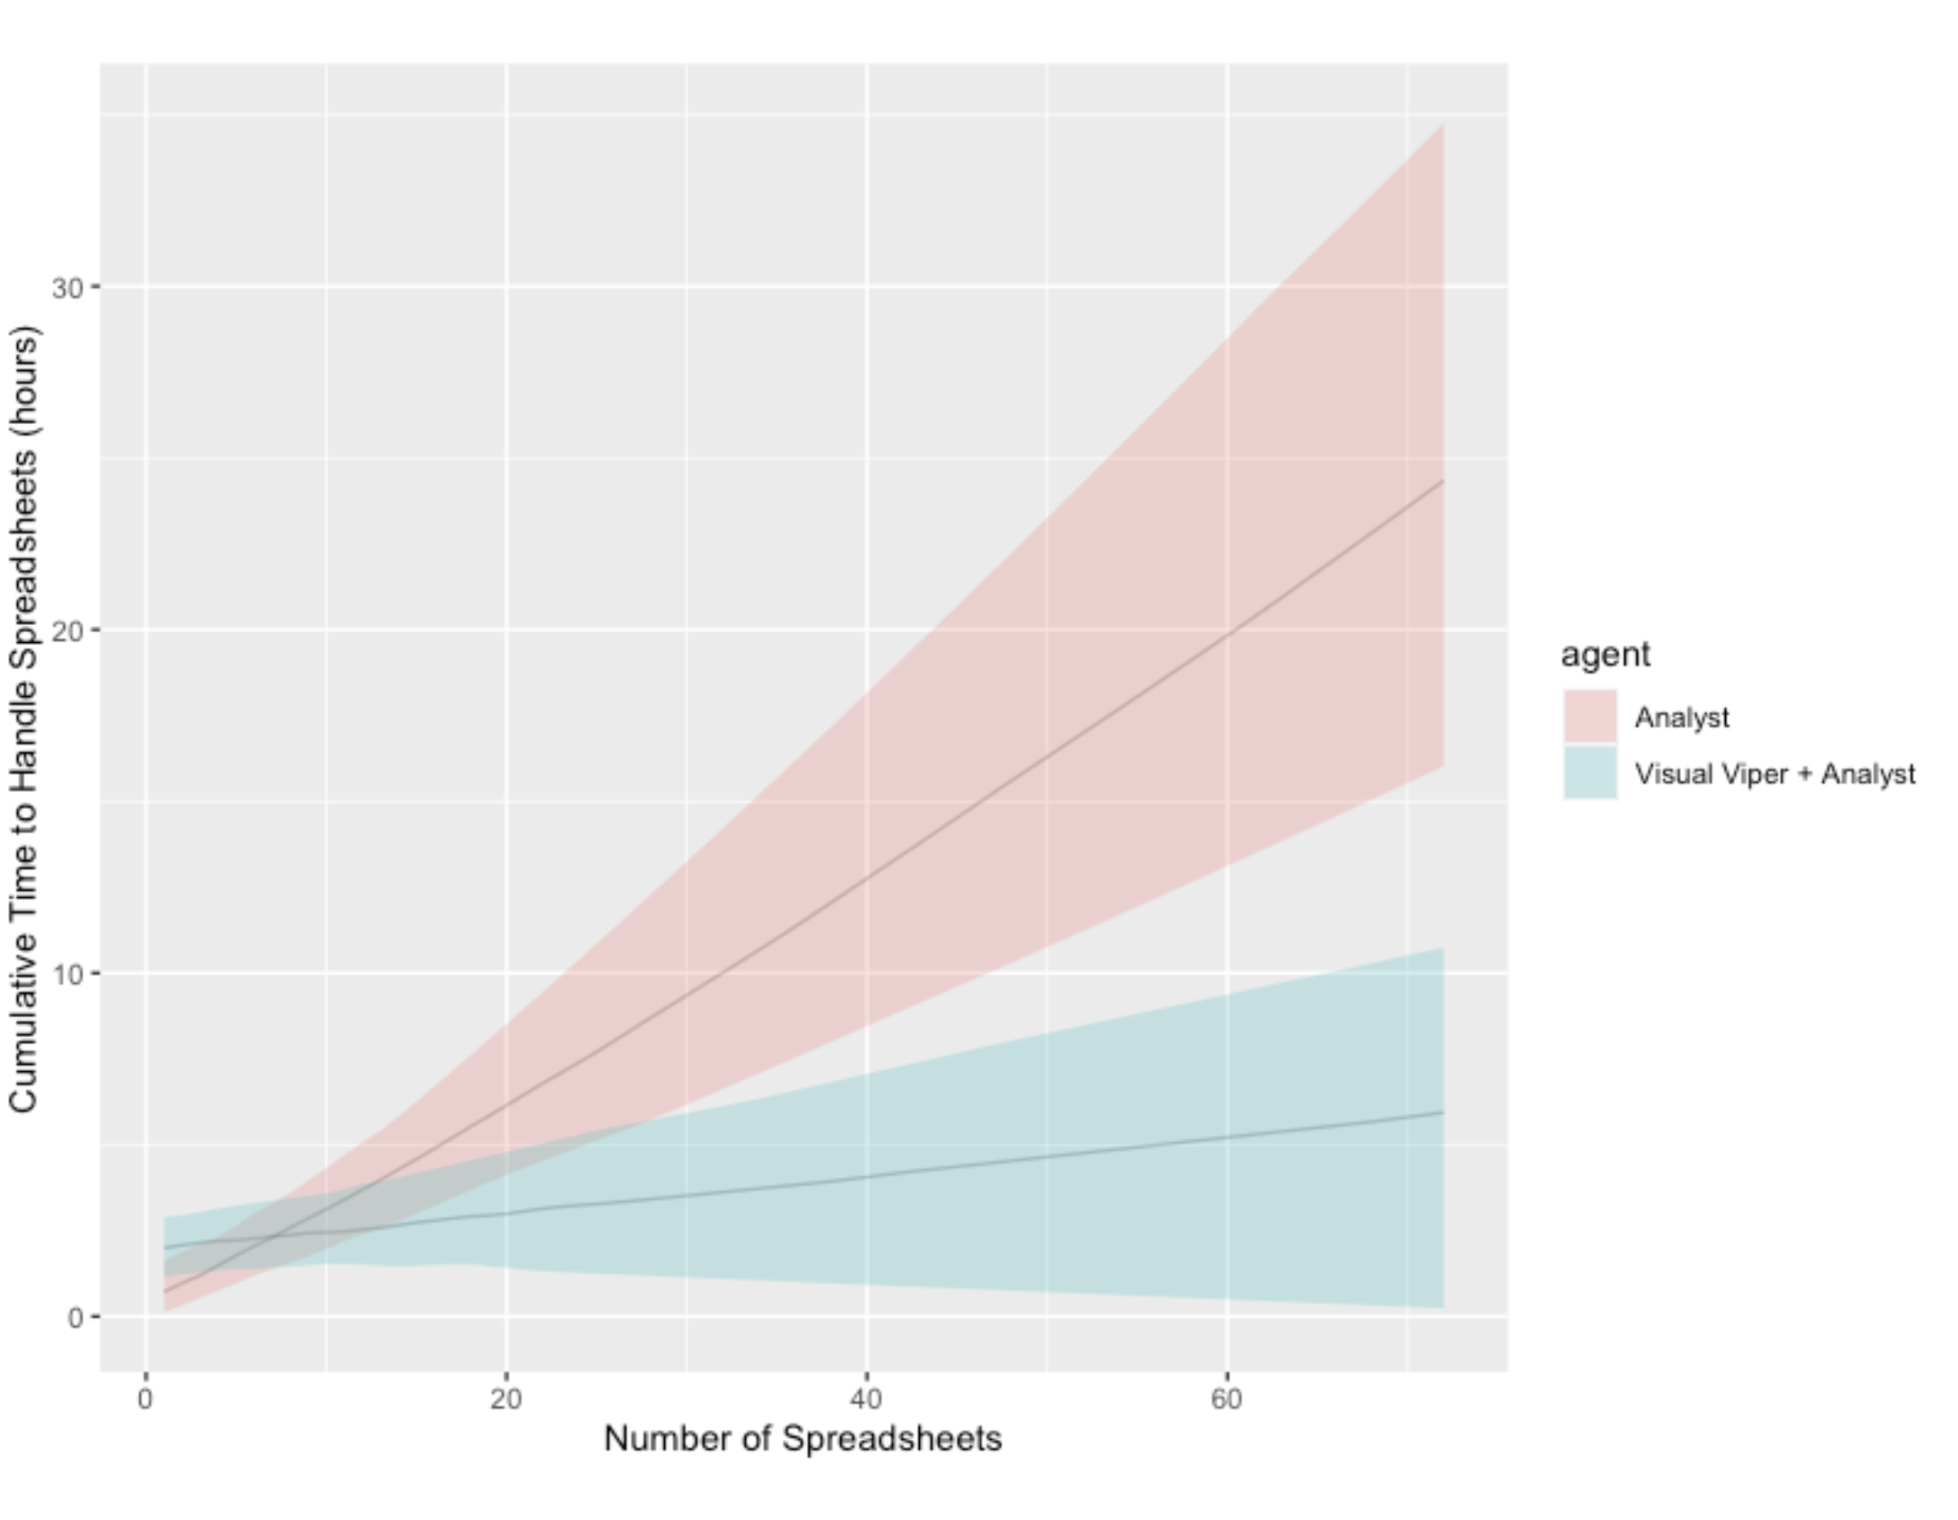
\includegraphics[width=\textwidth]{media/fig19.png}
  \caption{Cumulative Time to Handle Spreadsheets for Different Agents}
  \label{fig:time_sim}
\end{figure}

\section{Key Takeaways}\label{key-takeaways}

The data presented in Table \ref{tab:times} and Figure \ref{fig:time_sim} offer significant insights
into the operational efficiencies associated with the VV Python library
for chart creation in academic research. In particular, the differential
impact of using VV in comparison to manual methods becomes more
pronounced as the size of the project increases.

Figure \ref{fig:time_sim} illustrates the cumulative time required to process 72
spreadsheets for both a standalone analyst and an augmented system
involving both an analyst and VV. One of the striking observations is
the crossover point where VV starts to show a time advantage. While the
initial setup time for VV is significantly higher (2 hours compared to
0.5 hours for the analyst), the system starts to outperform the analyst
alone at around 8 spreadsheets. By the time 25 spreadsheets are
processed, the confidence intervals for the two methods no longer
overlap, signaling a clear advantage for VV.

Our adjusted metrics also account for factors like task fatigue and the
need for additional human verification of VV's outputs. Even after these
considerations, VV holds an advantage in larger projects, both in terms
of time efficiency and likely in terms of reduced human error owing to
fatigue.

Another significant aspect that adds complexity to this evaluation is
the dynamic nature of these data collection processes. Studies are
rarely static; they often require adjustments to the design or updating
of data. These changes necessitate updating the charts, perhaps multiple
times over the course of a study. While the initial setup is a one-time
task, adjustments and updates are recurring tasks that continue to
consume time. If the initial process is manual and lacks scalability,
these frequent updates can quickly become a resource-consuming
bottleneck. This is where the growing performance advantages of VV become particularly compelling. Our evaluation so far has
considered only a single iteration of a project with 72 spreadsheets. In
a dynamic study environment requiring frequent adjustments and updates,
the scalability advantages of VV could be even more pronounced. Each
update in a manual setting can be seen as an iteration that consumes
substantial time and resources. VV, which already shows performance
benefits in larger projects and single iterations, is likely to magnify
these advantages in the context of ongoing, multiple iterations.
Therefore, in a continually evolving study, the initial time investment
in setting up VV is likely to yield significant long-term savings.
